% Created by tikzDevice version 0.12.3.2 on 2022-02-07 12:38:14
% !TEX encoding = UTF-8 Unicode
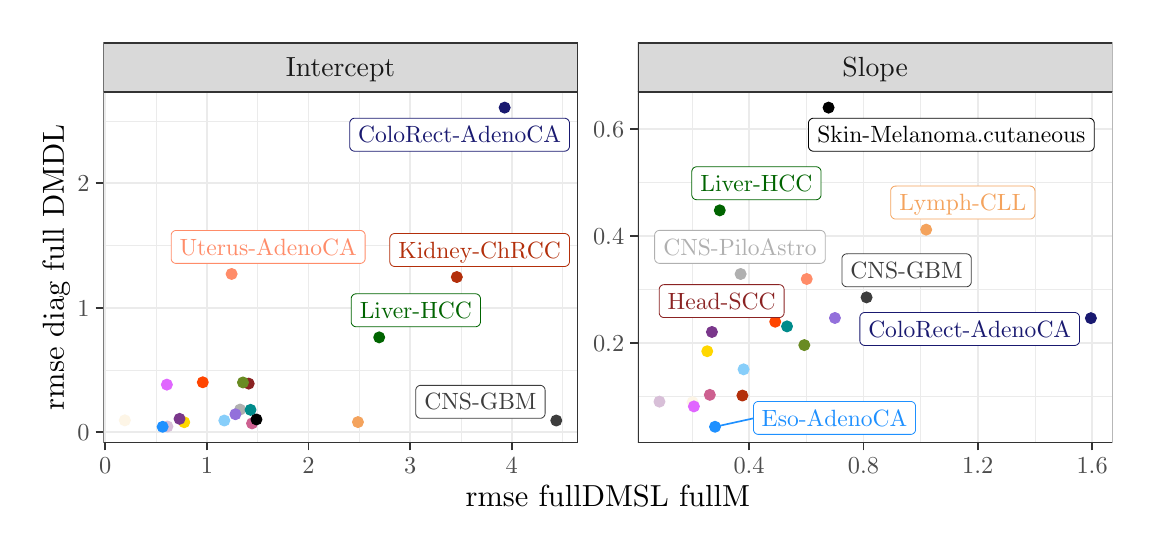
\begin{tikzpicture}[x=1pt,y=1pt]
\definecolor{fillColor}{RGB}{255,255,255}
\path[use as bounding box,fill=fillColor,fill opacity=0.00] (0,0) rectangle (397.48,180.67);
\begin{scope}
\path[clip] (  0.00,  0.00) rectangle (397.48,180.67);
\definecolor{drawColor}{RGB}{255,255,255}
\definecolor{fillColor}{RGB}{255,255,255}

\path[draw=drawColor,line width= 0.6pt,line join=round,line cap=round,fill=fillColor] (  0.00,  0.00) rectangle (397.48,180.68);
\end{scope}
\begin{scope}
\path[clip] ( 27.31, 30.69) rectangle (198.80,157.54);
\definecolor{fillColor}{RGB}{255,255,255}

\path[fill=fillColor] ( 27.31, 30.69) rectangle (198.80,157.54);
\definecolor{drawColor}{gray}{0.92}

\path[draw=drawColor,line width= 0.3pt,line join=round] ( 27.31, 56.98) --
	(198.80, 56.98);

\path[draw=drawColor,line width= 0.3pt,line join=round] ( 27.31,101.97) --
	(198.80,101.97);

\path[draw=drawColor,line width= 0.3pt,line join=round] ( 27.31,146.96) --
	(198.80,146.96);

\path[draw=drawColor,line width= 0.3pt,line join=round] ( 46.40, 30.69) --
	( 46.40,157.54);

\path[draw=drawColor,line width= 0.3pt,line join=round] ( 83.13, 30.69) --
	( 83.13,157.54);

\path[draw=drawColor,line width= 0.3pt,line join=round] (119.85, 30.69) --
	(119.85,157.54);

\path[draw=drawColor,line width= 0.3pt,line join=round] (156.58, 30.69) --
	(156.58,157.54);

\path[draw=drawColor,line width= 0.3pt,line join=round] (193.30, 30.69) --
	(193.30,157.54);

\path[draw=drawColor,line width= 0.6pt,line join=round] ( 27.31, 34.49) --
	(198.80, 34.49);

\path[draw=drawColor,line width= 0.6pt,line join=round] ( 27.31, 79.48) --
	(198.80, 79.48);

\path[draw=drawColor,line width= 0.6pt,line join=round] ( 27.31,124.46) --
	(198.80,124.46);

\path[draw=drawColor,line width= 0.6pt,line join=round] ( 28.04, 30.69) --
	( 28.04,157.54);

\path[draw=drawColor,line width= 0.6pt,line join=round] ( 64.76, 30.69) --
	( 64.76,157.54);

\path[draw=drawColor,line width= 0.6pt,line join=round] (101.49, 30.69) --
	(101.49,157.54);

\path[draw=drawColor,line width= 0.6pt,line join=round] (138.21, 30.69) --
	(138.21,157.54);

\path[draw=drawColor,line width= 0.6pt,line join=round] (174.94, 30.69) --
	(174.94,157.54);
\definecolor{drawColor}{RGB}{255,215,0}
\definecolor{fillColor}{RGB}{255,215,0}

\path[draw=drawColor,line width= 0.4pt,line join=round,line cap=round,fill=fillColor] ( 56.58, 38.09) circle (  1.96);
\definecolor{drawColor}{RGB}{205,96,144}
\definecolor{fillColor}{RGB}{205,96,144}

\path[draw=drawColor,line width= 0.4pt,line join=round,line cap=round,fill=fillColor] ( 81.07, 37.68) circle (  1.96);
\definecolor{drawColor}{gray}{0.24}
\definecolor{fillColor}{gray}{0.24}

\path[draw=drawColor,line width= 0.4pt,line join=round,line cap=round,fill=fillColor] (191.01, 38.71) circle (  1.96);
\definecolor{drawColor}{RGB}{216,191,216}
\definecolor{fillColor}{RGB}{216,191,216}

\path[draw=drawColor,line width= 0.4pt,line join=round,line cap=round,fill=fillColor] ( 50.49, 36.56) circle (  1.96);
\definecolor{drawColor}{gray}{0.69}
\definecolor{fillColor}{gray}{0.69}

\path[draw=drawColor,line width= 0.4pt,line join=round,line cap=round,fill=fillColor] ( 76.75, 42.67) circle (  1.96);
\definecolor{drawColor}{RGB}{25,25,112}
\definecolor{fillColor}{RGB}{25,25,112}

\path[draw=drawColor,line width= 0.4pt,line join=round,line cap=round,fill=fillColor] (172.35,151.78) circle (  1.96);
\definecolor{drawColor}{RGB}{30,144,255}
\definecolor{fillColor}{RGB}{30,144,255}

\path[draw=drawColor,line width= 0.4pt,line join=round,line cap=round,fill=fillColor] ( 48.77, 36.45) circle (  1.96);
\definecolor{drawColor}{RGB}{139,35,35}
\definecolor{fillColor}{RGB}{139,35,35}

\path[draw=drawColor,line width= 0.4pt,line join=round,line cap=round,fill=fillColor] ( 79.87, 52.05) circle (  1.96);
\definecolor{drawColor}{RGB}{179,47,11}
\definecolor{fillColor}{RGB}{179,47,11}

\path[draw=drawColor,line width= 0.4pt,line join=round,line cap=round,fill=fillColor] (155.07, 90.56) circle (  1.96);
\definecolor{drawColor}{RGB}{255,69,0}
\definecolor{fillColor}{RGB}{255,69,0}

\path[draw=drawColor,line width= 0.4pt,line join=round,line cap=round,fill=fillColor] ( 63.28, 52.53) circle (  1.96);
\definecolor{drawColor}{RGB}{0,100,0}
\definecolor{fillColor}{RGB}{0,100,0}

\path[draw=drawColor,line width= 0.4pt,line join=round,line cap=round,fill=fillColor] (127.02, 68.76) circle (  1.96);
\definecolor{drawColor}{RGB}{253,245,230}
\definecolor{fillColor}{RGB}{253,245,230}

\path[draw=drawColor,line width= 0.4pt,line join=round,line cap=round,fill=fillColor] ( 35.11, 38.78) circle (  1.96);
\definecolor{drawColor}{RGB}{105,139,34}
\definecolor{fillColor}{RGB}{105,139,34}

\path[draw=drawColor,line width= 0.4pt,line join=round,line cap=round,fill=fillColor] ( 77.80, 52.47) circle (  1.96);
\definecolor{drawColor}{RGB}{244,163,93}
\definecolor{fillColor}{RGB}{244,163,93}

\path[draw=drawColor,line width= 0.4pt,line join=round,line cap=round,fill=fillColor] (119.34, 38.15) circle (  1.96);
\definecolor{drawColor}{RGB}{0,139,139}
\definecolor{fillColor}{RGB}{0,139,139}

\path[draw=drawColor,line width= 0.4pt,line join=round,line cap=round,fill=fillColor] ( 80.53, 42.57) circle (  1.96);
\definecolor{drawColor}{RGB}{122,55,139}
\definecolor{fillColor}{RGB}{122,55,139}

\path[draw=drawColor,line width= 0.4pt,line join=round,line cap=round,fill=fillColor] ( 54.88, 39.32) circle (  1.96);
\definecolor{drawColor}{RGB}{224,102,255}
\definecolor{fillColor}{RGB}{224,102,255}

\path[draw=drawColor,line width= 0.4pt,line join=round,line cap=round,fill=fillColor] ( 50.30, 51.68) circle (  1.96);
\definecolor{drawColor}{RGB}{135,206,250}
\definecolor{fillColor}{RGB}{135,206,250}

\path[draw=drawColor,line width= 0.4pt,line join=round,line cap=round,fill=fillColor] ( 71.06, 38.71) circle (  1.96);
\definecolor{drawColor}{RGB}{0,0,0}
\definecolor{fillColor}{RGB}{0,0,0}

\path[draw=drawColor,line width= 0.4pt,line join=round,line cap=round,fill=fillColor] ( 82.67, 39.10) circle (  1.96);
\definecolor{drawColor}{RGB}{147,112,219}
\definecolor{fillColor}{RGB}{147,112,219}

\path[draw=drawColor,line width= 0.4pt,line join=round,line cap=round,fill=fillColor] ( 75.07, 40.98) circle (  1.96);
\definecolor{drawColor}{RGB}{255,140,105}
\definecolor{fillColor}{RGB}{255,140,105}

\path[draw=drawColor,line width= 0.4pt,line join=round,line cap=round,fill=fillColor] ( 73.69, 91.67) circle (  1.96);
\end{scope}
\begin{scope}
\path[clip] ( 27.31, 30.69) rectangle (198.80,157.54);
\definecolor{drawColor}{gray}{0.24}
\definecolor{fillColor}{RGB}{255,255,255}

\path[draw=drawColor,line width= 0.3pt,line join=round,line cap=round,fill=fillColor] (142.04, 39.52) --
	(185.17, 39.52) --
	(185.09, 39.52) --
	(185.38, 39.53) --
	(185.67, 39.59) --
	(185.94, 39.69) --
	(186.19, 39.84) --
	(186.42, 40.02) --
	(186.61, 40.24) --
	(186.77, 40.49) --
	(186.88, 40.75) --
	(186.95, 41.04) --
	(186.97, 41.33) --
	(186.97, 41.33) --
	(186.97, 49.61) --
	(186.97, 49.61) --
	(186.95, 49.90) --
	(186.88, 50.19) --
	(186.77, 50.45) --
	(186.61, 50.70) --
	(186.42, 50.92) --
	(186.19, 51.10) --
	(185.94, 51.25) --
	(185.67, 51.35) --
	(185.38, 51.41) --
	(185.17, 51.42) --
	(142.04, 51.42) --
	(142.26, 51.41) --
	(141.97, 51.42) --
	(141.68, 51.39) --
	(141.40, 51.30) --
	(141.14, 51.18) --
	(140.90, 51.01) --
	(140.69, 50.81) --
	(140.52, 50.58) --
	(140.38, 50.32) --
	(140.29, 50.05) --
	(140.24, 49.76) --
	(140.24, 49.61) --
	(140.24, 41.33) --
	(140.24, 41.47) --
	(140.24, 41.18) --
	(140.29, 40.89) --
	(140.38, 40.62) --
	(140.52, 40.36) --
	(140.69, 40.13) --
	(140.90, 39.93) --
	(141.14, 39.76) --
	(141.40, 39.64) --
	(141.68, 39.56) --
	(141.97, 39.52) --
	cycle;
\end{scope}
\begin{scope}
\path[clip] ( 27.31, 30.69) rectangle (198.80,157.54);
\definecolor{drawColor}{gray}{0.24}

\node[text=drawColor,anchor=base,inner sep=0pt, outer sep=0pt, scale=  0.85] at (163.60, 42.53) {CNS-GBM};
\definecolor{drawColor}{RGB}{25,25,112}
\definecolor{fillColor}{RGB}{255,255,255}

\path[draw=drawColor,line width= 0.3pt,line join=round,line cap=round,fill=fillColor] (118.18,136.04) --
	(193.96,136.04) --
	(193.89,136.04) --
	(194.18,136.05) --
	(194.46,136.11) --
	(194.74,136.21) --
	(194.99,136.36) --
	(195.21,136.54) --
	(195.41,136.76) --
	(195.56,137.00) --
	(195.68,137.27) --
	(195.75,137.55) --
	(195.77,137.84) --
	(195.77,137.84) --
	(195.77,146.13) --
	(195.77,146.13) --
	(195.75,146.42) --
	(195.68,146.70) --
	(195.56,146.97) --
	(195.41,147.22) --
	(195.21,147.44) --
	(194.99,147.62) --
	(194.74,147.76) --
	(194.46,147.87) --
	(194.18,147.93) --
	(193.96,147.94) --
	(118.18,147.94) --
	(118.40,147.93) --
	(118.11,147.94) --
	(117.82,147.90) --
	(117.54,147.82) --
	(117.28,147.70) --
	(117.04,147.53) --
	(116.83,147.33) --
	(116.66,147.10) --
	(116.52,146.84) --
	(116.43,146.56) --
	(116.38,146.28) --
	(116.38,146.13) --
	(116.38,137.84) --
	(116.38,137.99) --
	(116.38,137.70) --
	(116.43,137.41) --
	(116.52,137.14) --
	(116.66,136.88) --
	(116.83,136.65) --
	(117.04,136.44) --
	(117.28,136.28) --
	(117.54,136.16) --
	(117.82,136.07) --
	(118.11,136.04) --
	cycle;
\end{scope}
\begin{scope}
\path[clip] ( 27.31, 30.69) rectangle (198.80,157.54);
\definecolor{drawColor}{RGB}{25,25,112}

\node[text=drawColor,anchor=base,inner sep=0pt, outer sep=0pt, scale=  0.85] at (156.07,139.05) {ColoRect-AdenoCA};
\definecolor{drawColor}{RGB}{179,47,11}
\definecolor{fillColor}{RGB}{255,255,255}

\path[draw=drawColor,line width= 0.3pt,line join=round,line cap=round,fill=fillColor] (132.66, 94.38) --
	(193.98, 94.38) --
	(193.91, 94.38) --
	(194.20, 94.39) --
	(194.48, 94.45) --
	(194.75, 94.56) --
	(195.01, 94.70) --
	(195.23, 94.89) --
	(195.42, 95.10) --
	(195.58, 95.35) --
	(195.69, 95.62) --
	(195.76, 95.90) --
	(195.79, 96.19) --
	(195.79, 96.19) --
	(195.79,104.48) --
	(195.79,104.48) --
	(195.76,104.77) --
	(195.69,105.05) --
	(195.58,105.32) --
	(195.42,105.56) --
	(195.23,105.78) --
	(195.01,105.96) --
	(194.75,106.11) --
	(194.48,106.21) --
	(194.20,106.27) --
	(193.98,106.28) --
	(132.66,106.28) --
	(132.88,106.27) --
	(132.59,106.28) --
	(132.30,106.25) --
	(132.02,106.17) --
	(131.76,106.04) --
	(131.52,105.88) --
	(131.31,105.67) --
	(131.14,105.44) --
	(131.00,105.18) --
	(130.91,104.91) --
	(130.86,104.62) --
	(130.86,104.48) --
	(130.86, 96.19) --
	(130.86, 96.33) --
	(130.86, 96.04) --
	(130.91, 95.76) --
	(131.00, 95.48) --
	(131.14, 95.22) --
	(131.31, 94.99) --
	(131.52, 94.79) --
	(131.76, 94.62) --
	(132.02, 94.50) --
	(132.30, 94.42) --
	(132.59, 94.38) --
	cycle;
\end{scope}
\begin{scope}
\path[clip] ( 27.31, 30.69) rectangle (198.80,157.54);
\definecolor{drawColor}{RGB}{179,47,11}

\node[text=drawColor,anchor=base,inner sep=0pt, outer sep=0pt, scale=  0.85] at (163.32, 97.39) {Kidney-ChRCC};
\definecolor{drawColor}{RGB}{0,100,0}
\definecolor{fillColor}{RGB}{255,255,255}

\path[draw=drawColor,line width= 0.3pt,line join=round,line cap=round,fill=fillColor] (118.72, 72.60) --
	(161.80, 72.60) --
	(161.73, 72.60) --
	(162.02, 72.62) --
	(162.31, 72.67) --
	(162.58, 72.78) --
	(162.83, 72.92) --
	(163.06, 73.11) --
	(163.25, 73.32) --
	(163.40, 73.57) --
	(163.52, 73.84) --
	(163.59, 74.12) --
	(163.61, 74.41) --
	(163.61, 74.41) --
	(163.61, 82.70) --
	(163.61, 82.70) --
	(163.59, 82.99) --
	(163.52, 83.27) --
	(163.40, 83.54) --
	(163.25, 83.78) --
	(163.06, 84.00) --
	(162.83, 84.18) --
	(162.58, 84.33) --
	(162.31, 84.43) --
	(162.02, 84.49) --
	(161.80, 84.50) --
	(118.72, 84.50) --
	(118.93, 84.49) --
	(118.64, 84.50) --
	(118.35, 84.47) --
	(118.08, 84.39) --
	(117.81, 84.26) --
	(117.57, 84.10) --
	(117.36, 83.90) --
	(117.19, 83.66) --
	(117.05, 83.41) --
	(116.96, 83.13) --
	(116.92, 82.84) --
	(116.91, 82.70) --
	(116.91, 74.41) --
	(116.92, 74.55) --
	(116.92, 74.26) --
	(116.96, 73.98) --
	(117.05, 73.70) --
	(117.19, 73.44) --
	(117.36, 73.21) --
	(117.57, 73.01) --
	(117.81, 72.84) --
	(118.08, 72.72) --
	(118.35, 72.64) --
	(118.64, 72.60) --
	cycle;
\end{scope}
\begin{scope}
\path[clip] ( 27.31, 30.69) rectangle (198.80,157.54);
\definecolor{drawColor}{RGB}{0,100,0}

\node[text=drawColor,anchor=base,inner sep=0pt, outer sep=0pt, scale=  0.85] at (140.26, 75.61) {Liver-HCC};
\definecolor{drawColor}{RGB}{255,140,105}
\definecolor{fillColor}{RGB}{255,255,255}

\path[draw=drawColor,line width= 0.3pt,line join=round,line cap=round,fill=fillColor] ( 53.66, 95.49) --
	(120.14, 95.49) --
	(120.07, 95.49) --
	(120.36, 95.50) --
	(120.65, 95.56) --
	(120.92, 95.66) --
	(121.17, 95.81) --
	(121.40, 95.99) --
	(121.59, 96.21) --
	(121.74, 96.45) --
	(121.86, 96.72) --
	(121.93, 97.00) --
	(121.95, 97.29) --
	(121.95, 97.29) --
	(121.95,105.58) --
	(121.95,105.58) --
	(121.93,105.87) --
	(121.86,106.15) --
	(121.74,106.42) --
	(121.59,106.67) --
	(121.40,106.89) --
	(121.17,107.07) --
	(120.92,107.21) --
	(120.65,107.32) --
	(120.36,107.38) --
	(120.14,107.39) --
	( 53.66,107.39) --
	( 53.88,107.38) --
	( 53.59,107.39) --
	( 53.30,107.35) --
	( 53.02,107.27) --
	( 52.76,107.15) --
	( 52.52,106.98) --
	( 52.31,106.78) --
	( 52.13,106.55) --
	( 52.00,106.29) --
	( 51.90,106.01) --
	( 51.86,105.73) --
	( 51.85,105.58) --
	( 51.85, 97.29) --
	( 51.86, 97.44) --
	( 51.86, 97.15) --
	( 51.90, 96.86) --
	( 52.00, 96.59) --
	( 52.13, 96.33) --
	( 52.31, 96.10) --
	( 52.52, 95.89) --
	( 52.76, 95.73) --
	( 53.02, 95.60) --
	( 53.30, 95.52) --
	( 53.59, 95.49) --
	cycle;
\end{scope}
\begin{scope}
\path[clip] ( 27.31, 30.69) rectangle (198.80,157.54);
\definecolor{drawColor}{RGB}{255,140,105}

\node[text=drawColor,anchor=base,inner sep=0pt, outer sep=0pt, scale=  0.85] at ( 86.90, 98.50) {Uterus-AdenoCA};
\definecolor{drawColor}{gray}{0.20}

\path[draw=drawColor,line width= 0.6pt,line join=round,line cap=round] ( 27.31, 30.69) rectangle (198.80,157.54);
\end{scope}
\begin{scope}
\path[clip] (220.50, 30.69) rectangle (391.98,157.54);
\definecolor{fillColor}{RGB}{255,255,255}

\path[fill=fillColor] (220.50, 30.69) rectangle (391.98,157.54);
\definecolor{drawColor}{gray}{0.92}

\path[draw=drawColor,line width= 0.3pt,line join=round] (220.50, 47.35) --
	(391.98, 47.35);

\path[draw=drawColor,line width= 0.3pt,line join=round] (220.50, 86.03) --
	(391.98, 86.03);

\path[draw=drawColor,line width= 0.3pt,line join=round] (220.50,124.72) --
	(391.98,124.72);

\path[draw=drawColor,line width= 0.3pt,line join=round] (240.03, 30.69) --
	(240.03,157.54);

\path[draw=drawColor,line width= 0.3pt,line join=round] (281.35, 30.69) --
	(281.35,157.54);

\path[draw=drawColor,line width= 0.3pt,line join=round] (322.67, 30.69) --
	(322.67,157.54);

\path[draw=drawColor,line width= 0.3pt,line join=round] (363.98, 30.69) --
	(363.98,157.54);

\path[draw=drawColor,line width= 0.6pt,line join=round] (220.50, 66.69) --
	(391.98, 66.69);

\path[draw=drawColor,line width= 0.6pt,line join=round] (220.50,105.37) --
	(391.98,105.37);

\path[draw=drawColor,line width= 0.6pt,line join=round] (220.50,144.06) --
	(391.98,144.06);

\path[draw=drawColor,line width= 0.6pt,line join=round] (260.69, 30.69) --
	(260.69,157.54);

\path[draw=drawColor,line width= 0.6pt,line join=round] (302.01, 30.69) --
	(302.01,157.54);

\path[draw=drawColor,line width= 0.6pt,line join=round] (343.32, 30.69) --
	(343.32,157.54);

\path[draw=drawColor,line width= 0.6pt,line join=round] (384.64, 30.69) --
	(384.64,157.54);
\definecolor{drawColor}{RGB}{255,215,0}
\definecolor{fillColor}{RGB}{255,215,0}

\path[draw=drawColor,line width= 0.4pt,line join=round,line cap=round,fill=fillColor] (245.56, 63.75) circle (  1.96);
\definecolor{drawColor}{RGB}{205,96,144}
\definecolor{fillColor}{RGB}{205,96,144}

\path[draw=drawColor,line width= 0.4pt,line join=round,line cap=round,fill=fillColor] (246.49, 47.99) circle (  1.96);
\definecolor{drawColor}{gray}{0.24}
\definecolor{fillColor}{gray}{0.24}

\path[draw=drawColor,line width= 0.4pt,line join=round,line cap=round,fill=fillColor] (303.13, 83.21) circle (  1.96);
\definecolor{drawColor}{RGB}{216,191,216}
\definecolor{fillColor}{RGB}{216,191,216}

\path[draw=drawColor,line width= 0.4pt,line join=round,line cap=round,fill=fillColor] (228.29, 45.54) circle (  1.96);
\definecolor{drawColor}{gray}{0.69}
\definecolor{fillColor}{gray}{0.69}

\path[draw=drawColor,line width= 0.4pt,line join=round,line cap=round,fill=fillColor] (257.62, 91.66) circle (  1.96);
\definecolor{drawColor}{RGB}{25,25,112}
\definecolor{fillColor}{RGB}{25,25,112}

\path[draw=drawColor,line width= 0.4pt,line join=round,line cap=round,fill=fillColor] (384.19, 75.70) circle (  1.96);
\definecolor{drawColor}{RGB}{30,144,255}
\definecolor{fillColor}{RGB}{30,144,255}

\path[draw=drawColor,line width= 0.4pt,line join=round,line cap=round,fill=fillColor] (248.37, 36.45) circle (  1.96);
\definecolor{drawColor}{RGB}{139,35,35}
\definecolor{fillColor}{RGB}{139,35,35}

\path[draw=drawColor,line width= 0.4pt,line join=round,line cap=round,fill=fillColor] (237.54, 82.52) circle (  1.96);
\definecolor{drawColor}{RGB}{179,47,11}
\definecolor{fillColor}{RGB}{179,47,11}

\path[draw=drawColor,line width= 0.4pt,line join=round,line cap=round,fill=fillColor] (258.27, 47.74) circle (  1.96);
\definecolor{drawColor}{RGB}{255,69,0}
\definecolor{fillColor}{RGB}{255,69,0}

\path[draw=drawColor,line width= 0.4pt,line join=round,line cap=round,fill=fillColor] (270.12, 74.41) circle (  1.96);
\definecolor{drawColor}{RGB}{0,100,0}
\definecolor{fillColor}{RGB}{0,100,0}

\path[draw=drawColor,line width= 0.4pt,line join=round,line cap=round,fill=fillColor] (250.09,114.66) circle (  1.96);
\definecolor{drawColor}{RGB}{253,245,230}
\definecolor{fillColor}{RGB}{253,245,230}

\path[draw=drawColor,line width= 0.4pt,line join=round,line cap=round,fill=fillColor] (240.26, 45.34) circle (  1.96);
\definecolor{drawColor}{RGB}{105,139,34}
\definecolor{fillColor}{RGB}{105,139,34}

\path[draw=drawColor,line width= 0.4pt,line join=round,line cap=round,fill=fillColor] (280.64, 65.97) circle (  1.96);
\definecolor{drawColor}{RGB}{244,163,93}
\definecolor{fillColor}{RGB}{244,163,93}

\path[draw=drawColor,line width= 0.4pt,line join=round,line cap=round,fill=fillColor] (324.67,107.68) circle (  1.96);
\definecolor{drawColor}{RGB}{0,139,139}
\definecolor{fillColor}{RGB}{0,139,139}

\path[draw=drawColor,line width= 0.4pt,line join=round,line cap=round,fill=fillColor] (274.39, 72.73) circle (  1.96);
\definecolor{drawColor}{RGB}{122,55,139}
\definecolor{fillColor}{RGB}{122,55,139}

\path[draw=drawColor,line width= 0.4pt,line join=round,line cap=round,fill=fillColor] (247.25, 70.71) circle (  1.96);
\definecolor{drawColor}{RGB}{224,102,255}
\definecolor{fillColor}{RGB}{224,102,255}

\path[draw=drawColor,line width= 0.4pt,line join=round,line cap=round,fill=fillColor] (240.74, 43.81) circle (  1.96);
\definecolor{drawColor}{RGB}{135,206,250}
\definecolor{fillColor}{RGB}{135,206,250}

\path[draw=drawColor,line width= 0.4pt,line join=round,line cap=round,fill=fillColor] (258.69, 57.21) circle (  1.96);
\definecolor{drawColor}{RGB}{0,0,0}
\definecolor{fillColor}{RGB}{0,0,0}

\path[draw=drawColor,line width= 0.4pt,line join=round,line cap=round,fill=fillColor] (289.40,151.78) circle (  1.96);
\definecolor{drawColor}{RGB}{147,112,219}
\definecolor{fillColor}{RGB}{147,112,219}

\path[draw=drawColor,line width= 0.4pt,line join=round,line cap=round,fill=fillColor] (291.70, 75.77) circle (  1.96);
\definecolor{drawColor}{RGB}{255,140,105}
\definecolor{fillColor}{RGB}{255,140,105}

\path[draw=drawColor,line width= 0.4pt,line join=round,line cap=round,fill=fillColor] (281.51, 89.85) circle (  1.96);
\end{scope}
\begin{scope}
\path[clip] (220.50, 30.69) rectangle (391.98,157.54);
\definecolor{drawColor}{RGB}{30,144,255}

\path[draw=drawColor,line width= 0.6pt,line join=round,line cap=round] (262.26, 39.50) -- (249.44, 36.69);
\definecolor{drawColor}{gray}{0.24}
\definecolor{fillColor}{RGB}{255,255,255}

\path[draw=drawColor,line width= 0.3pt,line join=round,line cap=round,fill=fillColor] (296.04, 87.05) --
	(339.16, 87.05) --
	(339.09, 87.05) --
	(339.38, 87.06) --
	(339.66, 87.12) --
	(339.93, 87.22) --
	(340.19, 87.37) --
	(340.41, 87.55) --
	(340.60, 87.77) --
	(340.76, 88.02) --
	(340.87, 88.28) --
	(340.94, 88.57) --
	(340.97, 88.86) --
	(340.97, 88.86) --
	(340.97, 97.14) --
	(340.97, 97.14) --
	(340.94, 97.43) --
	(340.87, 97.72) --
	(340.76, 97.98) --
	(340.60, 98.23) --
	(340.41, 98.45) --
	(340.19, 98.63) --
	(339.93, 98.78) --
	(339.66, 98.88) --
	(339.38, 98.94) --
	(339.16, 98.95) --
	(296.04, 98.95) --
	(296.25, 98.94) --
	(295.96, 98.95) --
	(295.68, 98.91) --
	(295.40, 98.83) --
	(295.13, 98.71) --
	(294.89, 98.54) --
	(294.68, 98.34) --
	(294.51, 98.11) --
	(294.38, 97.85) --
	(294.28, 97.58) --
	(294.24, 97.29) --
	(294.23, 97.14) --
	(294.23, 88.86) --
	(294.24, 89.00) --
	(294.24, 88.71) --
	(294.28, 88.42) --
	(294.38, 88.15) --
	(294.51, 87.89) --
	(294.68, 87.66) --
	(294.89, 87.46) --
	(295.13, 87.29) --
	(295.40, 87.17) --
	(295.68, 87.09) --
	(295.96, 87.05) --
	cycle;
\end{scope}
\begin{scope}
\path[clip] (220.50, 30.69) rectangle (391.98,157.54);
\definecolor{drawColor}{gray}{0.24}

\node[text=drawColor,anchor=base,inner sep=0pt, outer sep=0pt, scale=  0.85] at (317.60, 90.06) {CNS-GBM};
\definecolor{drawColor}{gray}{0.69}
\definecolor{fillColor}{RGB}{255,255,255}

\path[draw=drawColor,line width= 0.3pt,line join=round,line cap=round,fill=fillColor] (228.35, 95.51) --
	(286.42, 95.51) --
	(286.35, 95.51) --
	(286.64, 95.53) --
	(286.92, 95.58) --
	(287.20, 95.69) --
	(287.45, 95.83) --
	(287.67, 96.02) --
	(287.87, 96.23) --
	(288.02, 96.48) --
	(288.13, 96.75) --
	(288.20, 97.03) --
	(288.23, 97.32) --
	(288.23, 97.32) --
	(288.23,105.61) --
	(288.23,105.61) --
	(288.20,105.90) --
	(288.13,106.18) --
	(288.02,106.45) --
	(287.87,106.69) --
	(287.67,106.91) --
	(287.45,107.09) --
	(287.20,107.24) --
	(286.92,107.34) --
	(286.64,107.40) --
	(286.42,107.41) --
	(228.35,107.41) --
	(228.57,107.40) --
	(228.28,107.41) --
	(227.99,107.38) --
	(227.71,107.30) --
	(227.45,107.17) --
	(227.21,107.01) --
	(227.00,106.80) --
	(226.82,106.57) --
	(226.69,106.31) --
	(226.60,106.04) --
	(226.55,105.75) --
	(226.54,105.61) --
	(226.54, 97.32) --
	(226.55, 97.46) --
	(226.55, 97.17) --
	(226.60, 96.89) --
	(226.69, 96.61) --
	(226.82, 96.35) --
	(227.00, 96.12) --
	(227.21, 95.92) --
	(227.45, 95.75) --
	(227.71, 95.63) --
	(227.99, 95.55) --
	(228.28, 95.51) --
	cycle;
\end{scope}
\begin{scope}
\path[clip] (220.50, 30.69) rectangle (391.98,157.54);
\definecolor{drawColor}{gray}{0.69}

\node[text=drawColor,anchor=base,inner sep=0pt, outer sep=0pt, scale=  0.85] at (257.39, 98.52) {CNS-PiloAstro};
\definecolor{drawColor}{RGB}{25,25,112}
\definecolor{fillColor}{RGB}{255,255,255}

\path[draw=drawColor,line width= 0.3pt,line join=round,line cap=round,fill=fillColor] (302.51, 65.85) --
	(378.29, 65.85) --
	(378.21, 65.85) --
	(378.51, 65.86) --
	(378.79, 65.92) --
	(379.06, 66.02) --
	(379.31, 66.17) --
	(379.54, 66.35) --
	(379.73, 66.57) --
	(379.89, 66.81) --
	(380.00, 67.08) --
	(380.07, 67.36) --
	(380.09, 67.65) --
	(380.09, 67.65) --
	(380.09, 75.94) --
	(380.09, 75.94) --
	(380.07, 76.23) --
	(380.00, 76.51) --
	(379.89, 76.78) --
	(379.73, 77.03) --
	(379.54, 77.25) --
	(379.31, 77.43) --
	(379.06, 77.57) --
	(378.79, 77.68) --
	(378.51, 77.74) --
	(378.29, 77.75) --
	(302.51, 77.75) --
	(302.73, 77.74) --
	(302.44, 77.75) --
	(302.15, 77.71) --
	(301.87, 77.63) --
	(301.61, 77.51) --
	(301.37, 77.34) --
	(301.16, 77.14) --
	(300.98, 76.91) --
	(300.85, 76.65) --
	(300.76, 76.37) --
	(300.71, 76.09) --
	(300.70, 75.94) --
	(300.70, 67.65) --
	(300.71, 67.80) --
	(300.71, 67.51) --
	(300.76, 67.22) --
	(300.85, 66.95) --
	(300.98, 66.69) --
	(301.16, 66.46) --
	(301.37, 66.25) --
	(301.61, 66.09) --
	(301.87, 65.96) --
	(302.15, 65.88) --
	(302.44, 65.85) --
	cycle;
\end{scope}
\begin{scope}
\path[clip] (220.50, 30.69) rectangle (391.98,157.54);
\definecolor{drawColor}{RGB}{25,25,112}

\node[text=drawColor,anchor=base,inner sep=0pt, outer sep=0pt, scale=  0.85] at (340.40, 68.86) {ColoRect-AdenoCA};
\definecolor{drawColor}{RGB}{30,144,255}
\definecolor{fillColor}{RGB}{255,255,255}

\path[draw=drawColor,line width= 0.3pt,line join=round,line cap=round,fill=fillColor] (264.07, 33.70) --
	(319.03, 33.70) --
	(318.96, 33.70) --
	(319.25, 33.71) --
	(319.54, 33.77) --
	(319.81, 33.87) --
	(320.06, 34.02) --
	(320.29, 34.20) --
	(320.48, 34.42) --
	(320.63, 34.66) --
	(320.75, 34.93) --
	(320.82, 35.21) --
	(320.84, 35.50) --
	(320.84, 35.50) --
	(320.84, 43.79) --
	(320.84, 43.79) --
	(320.82, 44.08) --
	(320.75, 44.36) --
	(320.63, 44.63) --
	(320.48, 44.88) --
	(320.29, 45.09) --
	(320.06, 45.28) --
	(319.81, 45.42) --
	(319.54, 45.53) --
	(319.25, 45.59) --
	(319.03, 45.60) --
	(264.07, 45.60) --
	(264.29, 45.59) --
	(264.00, 45.60) --
	(263.71, 45.56) --
	(263.43, 45.48) --
	(263.17, 45.36) --
	(262.93, 45.19) --
	(262.72, 44.99) --
	(262.54, 44.76) --
	(262.41, 44.50) --
	(262.32, 44.22) --
	(262.27, 43.94) --
	(262.26, 43.79) --
	(262.26, 35.50) --
	(262.27, 35.65) --
	(262.27, 35.36) --
	(262.32, 35.07) --
	(262.41, 34.80) --
	(262.54, 34.54) --
	(262.72, 34.31) --
	(262.93, 34.10) --
	(263.17, 33.94) --
	(263.43, 33.81) --
	(263.71, 33.73) --
	(264.00, 33.70) --
	cycle;
\end{scope}
\begin{scope}
\path[clip] (220.50, 30.69) rectangle (391.98,157.54);
\definecolor{drawColor}{RGB}{30,144,255}

\node[text=drawColor,anchor=base,inner sep=0pt, outer sep=0pt, scale=  0.85] at (291.55, 36.71) {Eso-AdenoCA};
\definecolor{drawColor}{RGB}{139,35,35}
\definecolor{fillColor}{RGB}{255,255,255}

\path[draw=drawColor,line width= 0.3pt,line join=round,line cap=round,fill=fillColor] (230.01, 75.91) --
	(271.53, 75.91) --
	(271.46, 75.91) --
	(271.75, 75.93) --
	(272.03, 75.98) --
	(272.30, 76.09) --
	(272.55, 76.23) --
	(272.78, 76.42) --
	(272.97, 76.63) --
	(273.13, 76.88) --
	(273.24, 77.15) --
	(273.31, 77.43) --
	(273.34, 77.72) --
	(273.34, 77.72) --
	(273.34, 86.01) --
	(273.34, 86.01) --
	(273.31, 86.30) --
	(273.24, 86.58) --
	(273.13, 86.85) --
	(272.97, 87.09) --
	(272.78, 87.31) --
	(272.55, 87.50) --
	(272.30, 87.64) --
	(272.03, 87.74) --
	(271.75, 87.80) --
	(271.53, 87.81) --
	(230.01, 87.81) --
	(230.22, 87.80) --
	(229.93, 87.81) --
	(229.64, 87.78) --
	(229.36, 87.70) --
	(229.10, 87.57) --
	(228.86, 87.41) --
	(228.65, 87.21) --
	(228.48, 86.97) --
	(228.34, 86.72) --
	(228.25, 86.44) --
	(228.20, 86.15) --
	(228.20, 86.01) --
	(228.20, 77.72) --
	(228.20, 77.87) --
	(228.20, 77.57) --
	(228.25, 77.29) --
	(228.34, 77.01) --
	(228.48, 76.75) --
	(228.65, 76.52) --
	(228.86, 76.32) --
	(229.10, 76.16) --
	(229.36, 76.03) --
	(229.64, 75.95) --
	(229.93, 75.91) --
	cycle;
\end{scope}
\begin{scope}
\path[clip] (220.50, 30.69) rectangle (391.98,157.54);
\definecolor{drawColor}{RGB}{139,35,35}

\node[text=drawColor,anchor=base,inner sep=0pt, outer sep=0pt, scale=  0.85] at (250.77, 78.92) {Head-SCC};
\definecolor{drawColor}{RGB}{0,100,0}
\definecolor{fillColor}{RGB}{255,255,255}

\path[draw=drawColor,line width= 0.3pt,line join=round,line cap=round,fill=fillColor] (241.79,118.50) --
	(284.87,118.50) --
	(284.80,118.50) --
	(285.09,118.51) --
	(285.38,118.57) --
	(285.65,118.68) --
	(285.90,118.82) --
	(286.13,119.01) --
	(286.32,119.22) --
	(286.47,119.47) --
	(286.59,119.74) --
	(286.66,120.02) --
	(286.68,120.31) --
	(286.68,120.31) --
	(286.68,128.60) --
	(286.68,128.60) --
	(286.66,128.89) --
	(286.59,129.17) --
	(286.47,129.44) --
	(286.32,129.68) --
	(286.13,129.90) --
	(285.90,130.08) --
	(285.65,130.23) --
	(285.38,130.33) --
	(285.09,130.39) --
	(284.87,130.40) --
	(241.79,130.40) --
	(242.01,130.39) --
	(241.71,130.40) --
	(241.43,130.37) --
	(241.15,130.29) --
	(240.88,130.16) --
	(240.64,130.00) --
	(240.43,129.79) --
	(240.26,129.56) --
	(240.13,129.30) --
	(240.03,129.03) --
	(239.99,128.74) --
	(239.98,128.60) --
	(239.98,120.31) --
	(239.99,120.45) --
	(239.99,120.16) --
	(240.03,119.88) --
	(240.13,119.60) --
	(240.26,119.34) --
	(240.43,119.11) --
	(240.64,118.91) --
	(240.88,118.74) --
	(241.15,118.62) --
	(241.43,118.54) --
	(241.71,118.50) --
	cycle;
\end{scope}
\begin{scope}
\path[clip] (220.50, 30.69) rectangle (391.98,157.54);
\definecolor{drawColor}{RGB}{0,100,0}

\node[text=drawColor,anchor=base,inner sep=0pt, outer sep=0pt, scale=  0.85] at (263.33,121.51) {Liver-HCC};
\definecolor{drawColor}{RGB}{244,163,93}
\definecolor{fillColor}{RGB}{255,255,255}

\path[draw=drawColor,line width= 0.3pt,line join=round,line cap=round,fill=fillColor] (313.65,111.53) --
	(362.17,111.53) --
	(362.10,111.53) --
	(362.39,111.54) --
	(362.67,111.60) --
	(362.94,111.70) --
	(363.20,111.85) --
	(363.42,112.03) --
	(363.61,112.25) --
	(363.77,112.49) --
	(363.88,112.76) --
	(363.95,113.04) --
	(363.98,113.33) --
	(363.98,113.33) --
	(363.98,121.62) --
	(363.98,121.62) --
	(363.95,121.91) --
	(363.88,122.19) --
	(363.77,122.46) --
	(363.61,122.71) --
	(363.42,122.92) --
	(363.20,123.11) --
	(362.94,123.25) --
	(362.67,123.36) --
	(362.39,123.41) --
	(362.17,123.43) --
	(313.65,123.43) --
	(313.87,123.41) --
	(313.58,123.43) --
	(313.29,123.39) --
	(313.01,123.31) --
	(312.75,123.19) --
	(312.51,123.02) --
	(312.30,122.82) --
	(312.13,122.59) --
	(311.99,122.33) --
	(311.90,122.05) --
	(311.85,121.77) --
	(311.85,121.62) --
	(311.85,113.33) --
	(311.85,113.48) --
	(311.85,113.19) --
	(311.90,112.90) --
	(311.99,112.63) --
	(312.13,112.37) --
	(312.30,112.14) --
	(312.51,111.93) --
	(312.75,111.77) --
	(313.01,111.64) --
	(313.29,111.56) --
	(313.58,111.53) --
	cycle;
\end{scope}
\begin{scope}
\path[clip] (220.50, 30.69) rectangle (391.98,157.54);
\definecolor{drawColor}{RGB}{244,163,93}

\node[text=drawColor,anchor=base,inner sep=0pt, outer sep=0pt, scale=  0.85] at (337.91,114.54) {Lymph-CLL};
\definecolor{drawColor}{RGB}{0,0,0}
\definecolor{fillColor}{RGB}{255,255,255}

\path[draw=drawColor,line width= 0.3pt,line join=round,line cap=round,fill=fillColor] (283.94,136.03) --
	(383.59,136.03) --
	(383.52,136.03) --
	(383.81,136.05) --
	(384.09,136.10) --
	(384.37,136.21) --
	(384.62,136.35) --
	(384.84,136.54) --
	(385.04,136.75) --
	(385.19,137.00) --
	(385.31,137.27) --
	(385.37,137.55) --
	(385.40,137.84) --
	(385.40,137.84) --
	(385.40,146.13) --
	(385.40,146.13) --
	(385.37,146.42) --
	(385.31,146.70) --
	(385.19,146.97) --
	(385.04,147.21) --
	(384.84,147.43) --
	(384.62,147.61) --
	(384.37,147.76) --
	(384.09,147.86) --
	(383.81,147.92) --
	(383.59,147.93) --
	(283.94,147.93) --
	(284.16,147.92) --
	(283.87,147.93) --
	(283.58,147.90) --
	(283.30,147.82) --
	(283.04,147.69) --
	(282.80,147.53) --
	(282.59,147.33) --
	(282.42,147.09) --
	(282.28,146.84) --
	(282.19,146.56) --
	(282.14,146.27) --
	(282.14,146.13) --
	(282.14,137.84) --
	(282.14,137.98) --
	(282.14,137.69) --
	(282.19,137.41) --
	(282.28,137.13) --
	(282.42,136.87) --
	(282.59,136.64) --
	(282.80,136.44) --
	(283.04,136.27) --
	(283.30,136.15) --
	(283.58,136.07) --
	(283.87,136.03) --
	cycle;
\end{scope}
\begin{scope}
\path[clip] (220.50, 30.69) rectangle (391.98,157.54);
\definecolor{drawColor}{RGB}{0,0,0}

\node[text=drawColor,anchor=base,inner sep=0pt, outer sep=0pt, scale=  0.85] at (333.77,139.04) {Skin-Melanoma.cutaneous};
\definecolor{drawColor}{gray}{0.20}

\path[draw=drawColor,line width= 0.6pt,line join=round,line cap=round] (220.50, 30.69) rectangle (391.98,157.54);
\end{scope}
\begin{scope}
\path[clip] ( 27.31,157.54) rectangle (198.80,175.17);
\definecolor{drawColor}{gray}{0.20}
\definecolor{fillColor}{gray}{0.85}

\path[draw=drawColor,line width= 0.6pt,line join=round,line cap=round,fill=fillColor] ( 27.31,157.54) rectangle (198.80,175.17);
\definecolor{drawColor}{gray}{0.10}

\node[text=drawColor,anchor=base,inner sep=0pt, outer sep=0pt, scale=  1.00] at (113.06,162.92) {Intercept};
\end{scope}
\begin{scope}
\path[clip] (220.50,157.54) rectangle (391.98,175.17);
\definecolor{drawColor}{gray}{0.20}
\definecolor{fillColor}{gray}{0.85}

\path[draw=drawColor,line width= 0.6pt,line join=round,line cap=round,fill=fillColor] (220.50,157.54) rectangle (391.98,175.17);
\definecolor{drawColor}{gray}{0.10}

\node[text=drawColor,anchor=base,inner sep=0pt, outer sep=0pt, scale=  1.00] at (306.24,162.92) {Slope};
\end{scope}
\begin{scope}
\path[clip] (  0.00,  0.00) rectangle (397.48,180.67);
\definecolor{drawColor}{gray}{0.20}

\path[draw=drawColor,line width= 0.6pt,line join=round] ( 28.04, 27.94) --
	( 28.04, 30.69);

\path[draw=drawColor,line width= 0.6pt,line join=round] ( 64.76, 27.94) --
	( 64.76, 30.69);

\path[draw=drawColor,line width= 0.6pt,line join=round] (101.49, 27.94) --
	(101.49, 30.69);

\path[draw=drawColor,line width= 0.6pt,line join=round] (138.21, 27.94) --
	(138.21, 30.69);

\path[draw=drawColor,line width= 0.6pt,line join=round] (174.94, 27.94) --
	(174.94, 30.69);
\end{scope}
\begin{scope}
\path[clip] (  0.00,  0.00) rectangle (397.48,180.67);
\definecolor{drawColor}{gray}{0.30}

\node[text=drawColor,anchor=base,inner sep=0pt, outer sep=0pt, scale=  0.88] at ( 28.04, 19.68) {0};

\node[text=drawColor,anchor=base,inner sep=0pt, outer sep=0pt, scale=  0.88] at ( 64.76, 19.68) {1};

\node[text=drawColor,anchor=base,inner sep=0pt, outer sep=0pt, scale=  0.88] at (101.49, 19.68) {2};

\node[text=drawColor,anchor=base,inner sep=0pt, outer sep=0pt, scale=  0.88] at (138.21, 19.68) {3};

\node[text=drawColor,anchor=base,inner sep=0pt, outer sep=0pt, scale=  0.88] at (174.94, 19.68) {4};
\end{scope}
\begin{scope}
\path[clip] (  0.00,  0.00) rectangle (397.48,180.67);
\definecolor{drawColor}{gray}{0.20}

\path[draw=drawColor,line width= 0.6pt,line join=round] (260.69, 27.94) --
	(260.69, 30.69);

\path[draw=drawColor,line width= 0.6pt,line join=round] (302.01, 27.94) --
	(302.01, 30.69);

\path[draw=drawColor,line width= 0.6pt,line join=round] (343.32, 27.94) --
	(343.32, 30.69);

\path[draw=drawColor,line width= 0.6pt,line join=round] (384.64, 27.94) --
	(384.64, 30.69);
\end{scope}
\begin{scope}
\path[clip] (  0.00,  0.00) rectangle (397.48,180.67);
\definecolor{drawColor}{gray}{0.30}

\node[text=drawColor,anchor=base,inner sep=0pt, outer sep=0pt, scale=  0.88] at (260.69, 19.68) {0.4};

\node[text=drawColor,anchor=base,inner sep=0pt, outer sep=0pt, scale=  0.88] at (302.01, 19.68) {0.8};

\node[text=drawColor,anchor=base,inner sep=0pt, outer sep=0pt, scale=  0.88] at (343.32, 19.68) {1.2};

\node[text=drawColor,anchor=base,inner sep=0pt, outer sep=0pt, scale=  0.88] at (384.64, 19.68) {1.6};
\end{scope}
\begin{scope}
\path[clip] (  0.00,  0.00) rectangle (397.48,180.67);
\definecolor{drawColor}{gray}{0.30}

\node[text=drawColor,anchor=base east,inner sep=0pt, outer sep=0pt, scale=  0.88] at (215.55, 63.66) {0.2};

\node[text=drawColor,anchor=base east,inner sep=0pt, outer sep=0pt, scale=  0.88] at (215.55,102.34) {0.4};

\node[text=drawColor,anchor=base east,inner sep=0pt, outer sep=0pt, scale=  0.88] at (215.55,141.03) {0.6};
\end{scope}
\begin{scope}
\path[clip] (  0.00,  0.00) rectangle (397.48,180.67);
\definecolor{drawColor}{gray}{0.20}

\path[draw=drawColor,line width= 0.6pt,line join=round] (217.75, 66.69) --
	(220.50, 66.69);

\path[draw=drawColor,line width= 0.6pt,line join=round] (217.75,105.37) --
	(220.50,105.37);

\path[draw=drawColor,line width= 0.6pt,line join=round] (217.75,144.06) --
	(220.50,144.06);
\end{scope}
\begin{scope}
\path[clip] (  0.00,  0.00) rectangle (397.48,180.67);
\definecolor{drawColor}{gray}{0.30}

\node[text=drawColor,anchor=base east,inner sep=0pt, outer sep=0pt, scale=  0.88] at ( 22.36, 31.46) {0};

\node[text=drawColor,anchor=base east,inner sep=0pt, outer sep=0pt, scale=  0.88] at ( 22.36, 76.45) {1};

\node[text=drawColor,anchor=base east,inner sep=0pt, outer sep=0pt, scale=  0.88] at ( 22.36,121.43) {2};
\end{scope}
\begin{scope}
\path[clip] (  0.00,  0.00) rectangle (397.48,180.67);
\definecolor{drawColor}{gray}{0.20}

\path[draw=drawColor,line width= 0.6pt,line join=round] ( 24.56, 34.49) --
	( 27.31, 34.49);

\path[draw=drawColor,line width= 0.6pt,line join=round] ( 24.56, 79.48) --
	( 27.31, 79.48);

\path[draw=drawColor,line width= 0.6pt,line join=round] ( 24.56,124.46) --
	( 27.31,124.46);
\end{scope}
\begin{scope}
\path[clip] (  0.00,  0.00) rectangle (397.48,180.67);
\definecolor{drawColor}{RGB}{0,0,0}

\node[text=drawColor,anchor=base,inner sep=0pt, outer sep=0pt, scale=  1.10] at (209.65,  7.64) {rmse fullDMSL fullM};
\end{scope}
\begin{scope}
\path[clip] (  0.00,  0.00) rectangle (397.48,180.67);
\definecolor{drawColor}{RGB}{0,0,0}

\node[text=drawColor,rotate= 90.00,anchor=base,inner sep=0pt, outer sep=0pt, scale=  1.10] at ( 13.08, 94.11) {rmse diag full DMDL};
\end{scope}
\end{tikzpicture}
